\documentclass{article}
    % General document formatting
    \usepackage[margin=0.7in]{geometry}
    \usepackage[parfill]{parskip}
    \usepackage[utf8]{inputenc}
    
    % Related to math
    \usepackage{amsmath,amssymb,amsfonts,amsthm}
\usepackage{graphicx}
%\usepackage{subfig}
%\usepackage{subfigure}
\usepackage{caption}
\usepackage{subcaption}
\usepackage{listings}
\usepackage{braket}
\usepackage{gensymb}
\usepackage[percent]{overpic}
\usepackage{xcolor,varwidth}
\usepackage{enumerate}

\usepackage{titling}
%\usepackage{lipsum}

\usepackage{titlesec}

\titleformat*{\section}{\large\bfseries}
\titleformat*{\subsection}{\large\bfseries}
%\titleformat*{\subsubsection}{\large\bfseries}
%\titleformat*{\paragraph}{\large\bfseries}
%\titleformat*{\subparagraph}{\large\bfseries}
\titlespacing\section{0pt}{2pt plus 2pt minus 2pt}{0pt plus 2pt minus 2pt}
\titlespacing\subsection{0pt}{12pt plus 4pt minus 2pt}{0pt plus 2pt minus 2pt}
\titlespacing\subsubsection{0pt}{12pt plus 4pt minus 2pt}{0pt plus 2pt minus 2pt}

\pretitle{\begin{center}\large\bfseries}
\posttitle{\par\end{center}\vskip 0.01em}
\preauthor{\begin{center}\Large\ttfamily}
\postauthor{\end{center}}
\predate{\par\normalsize\centering}
\postdate{\par}

\begin{document}

%\maketitle

\begin{center}
\textbf{\LARGE{\centering{Deep Learning}}}\\

\textit{USN: 303039534}\\
\end{center}

\section{Perceptron}

We implement a two-state perceptron with weights \textbf{w} and inputs \textbf{u} as described in Dayan and Abbott such that the state $v$ of the perceptron is given by
\begin{equation}
\begin{split}
+1 \,\,\, if \,\,\,  {\bf w \cdot u} - \gamma > 0 \\
-1 \,\,\, if \,\,\,  {\bf w \cdot u} - \gamma < 0
\end{split}
\end{equation}
Where $\gamma$ is a threshold parameter.

We note that for the present task of classifying inputs according to whether their sum is positive or negative, the state of the perceptron is undefined in the case where our 10-element input vector has a sum of 0.
We can approch this problem in two ways. Either we consider 0 as a separate state and train the perceptron on a 3-way classification problem. Otherwise, we arbitrarily assign state 0 to either the set of positive-sum or negative-sum input vectors. Since a perceptron in its strictest sense must be a binary classifier of binary inputs, we opt for the latter solution and arbitrarily classify zero-sum input vectors as belonging to the +1 state.

We train this perceptron using three different learning rules as also described in Dayan and Abbott.
\begin{enumerate}
\item
The Hebbian learning rule given in equation \ref{eq:hebbian}
\begin{equation}\label{eq:hebbian}
{\bf w} = \dfrac{1}{N_\mu} \sum_{m = 1}^{N_S}{v^m {\bf u}^m}
\end{equation}
Here $N_\mu$ is the dimensionality of the space, $N_S$ is the number of input patterns, and $v^m$ is the desired output for pattern $m$ with input ${\bf u}^m$. Note that this learning rule contains no method for updating $\gamma$ which is thus fixed at 0 in the present implementation.

\item
The perceptron learning rule given in equation \ref{eq:perceptron}
\begin{equation}\label{eq:perceptron}
{\bf w} \rightarrow {\bf w} + \dfrac{\epsilon_w}{2}(v^m - v({\bf u}^m)) {\bf u}^m
\end{equation}
\begin{equation}
\gamma \rightarrow \gamma - \dfrac{\epsilon_w}{2}(v^m - v({\bf u}^m))
\end{equation}
Here $\epsilon_w$ is the learning rate,  $v({\bf u}^m)$ is the predicted perceptron state for input $m$, and the other parameters are as above.

\item
The delta learning rule given in equation \ref{eq:delta}.
\begin{equation}\label{eq:delta}
{\bf w} \rightarrow {\bf w} - \epsilon_w \nabla_w E
\end{equation}
The penalty function we are trying to minimize is given by
\begin{equation}
E = \dfrac{1}{2} \sum_{m=1}^{N_S}{(v^m-v({\bf u}^m))^2}
\end{equation}
Writing $v({\bf u}^m) = \text{sign}( {\bf w} \cdot {\bf u}^m - \gamma) \approx {\bf w} \cdot {\bf u}^m - \gamma $ we can write out the derivative explicitly as
\begin{equation}
 \nabla_w E =- \sum_{m=1}^{N_S}{(v^m-v({\bf u}^m)) \nabla_w E({\bf w} \cdot {\bf u}^m)} = - \sum_{m=1}^{N_S}{(v^m-v({\bf u}^m)) {\bf u}^m}
\end{equation}
\begin{equation}
 \nabla_\gamma E = \sum_{m=1}^{N_S}{(v^m-v({\bf u}^m))}
\end{equation}
This is entirely equivalent to a batch-version of the perceptron learning rule, and we will therefore observe similar behavior for the two learning rules in our analyses.
\end{enumerate}

For the perceptron and delta learning rules, we let $\epsilon_w = 0.01$ for all analyses and terminate learning once the norm of the change in weights is less than $10^{-6}$ per iteration. Altering these parameters within a reasonable range was not found to affect the performance of the networks.

For an initial investigation of how the three learning rules perform on this problem, we assess performance as a function of the number of training patterns N and plot the result in figure \ref{fig:performance_sum}. The total number of possible input patterns is $2^{10} = 1024$, and varying N from 1 to 400 we observe convergence at $N > 250$. To quantify the performance for each N, we train 10 separate networks on N randomly generated patterns, calculate the fraction of 1000 randomly generated query patterns that are categorized correctly, and average this value over the 10 trials.

\begin{figure}[h]
	\centering
	\begin{subfigure}[t]{0.60\linewidth}
		\centering
		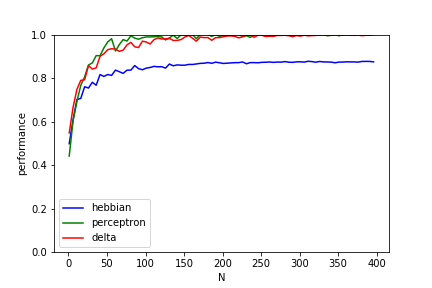
\includegraphics[width = 1.0\linewidth, trim={10 5 40 30}, clip=true]{figures/compare_sum.png}
		%\subcaption{Reference}
		%\label{}	
	\end{subfigure}%
\caption{Performance in the sum-classification task as a function of the number of training vectors N for the Hebbian, perceptron and delta learning rules.}
\label{fig:performance_sum}
\end{figure}

As expected from the considerations above, the perceptron and delta learning rules exhibit very similar performance, and both learning rules lead to perfect classification when $N \geq 250$. This is expected since it can be shown mathematically that the perceptron learning rule will converge to a perfect classifier when the problem is linearly separable (Dayan and Abbott).

As expected, the Hebbian learning rule performs somewhat worse as it does not explicitly optimize our utility function and thus converges to a performance of 87\%. We can gain further insights into the failure modes of the networks trained by the different methods by assessing their ability to classify inputs specifically when the input vectors contain a particular number $n$ of positive elements and $10-n$ negative elements (figure \ref{fig:nplus}).


\begin{figure}[h]
	\centering
	\begin{subfigure}[t]{0.32\linewidth}
		\centering
		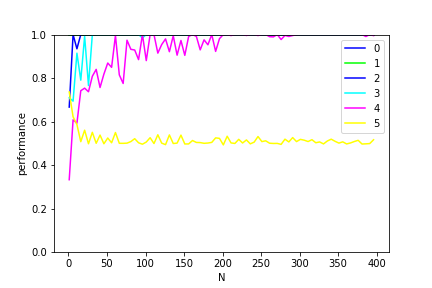
\includegraphics[width = 1.0\linewidth, trim={10 5 40 30}, clip=true]{figures/nplus_heb.png}
		\subcaption{Hebbian learning}
		%\label{}	
	\end{subfigure}%
	\hspace{0.01 \linewidth}
	\begin{subfigure}[t]{0.32\linewidth}
		\centering
		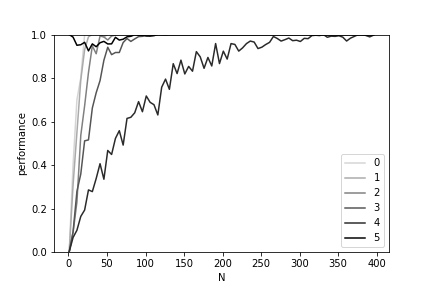
\includegraphics[width = 1.0\linewidth, trim={10 5 40 30}, clip=true]{figures/nplus_perceptron.png}
		\subcaption{Perceptron learning}	
		%\label{}
	\end{subfigure}%
	\hspace{0.01 \linewidth}
	\begin{subfigure}[t]{0.32\linewidth}
		\centering
		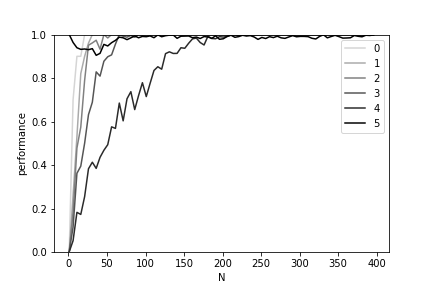
\includegraphics[width = 1.0\linewidth, trim={10 5 40 30}, clip=true]{figures/nplus_delta.png}
		\subcaption{Delta learning}	
		%\label{}
	\end{subfigure}%
\caption{Performance of a perceptron in the sum-classification task depending on the number of positive elements in the 10-element input vector. Learning curves are coloured from lighter to darker as the number of positive elements incnreases from 0 to 6.}
\label{fig:nplus}
\end{figure}

\newpage

We see that all three learning rules perform the worst when classifying inputs with 5 positive elements, followed by $n=4$ for the delta and perceptron learning rules with $n=4$ and $n=6$ being equally hard for the Hebbian network. The Hebbian network has a performance of only 50\% for $n=5$, but once we realize that the Hebbian network has $\gamma=0$ this is not surprising. The expected value of a given input element is $\braket{u_i^m} = 0$ for $n=5$ and the expected value $\braket{v^m*u_i^m} > 0$ for $n \neq 5$ and identical for all i. We thus expect the Hebbian weights to approach a scaled vector of ones as N increases, which is also observed empirically. With $\gamma = 0$, this leads to correct classification when $n \neq 5$ but random classification of the $n=5$ case depending only on the noise in the input data. Indeed the overall converged performance of 87\% for the Hebbian network arises from a perfect performance on inputs with $n \neq 5$ and 50\% success for the 25\% of inputs for which $n=5$. If we artificially imposed a negative gamma, we would therefore likely get better performance for the Hebbian network. Performance is worst for $n=5$ and $n=4$ in the perceptron and delta networks since these are the cases separating the two output categories and thus most easily affected by noise in the training data.

Having considered the relatively simple sum-classification task where $v = \text{sign}(\sum_i{u_i})$ we now proceed to the more complex task of classifying 10-element input vectors according to the product of their elements $v = \text{sign}(\prod_i{u_i})$. The performance in this task for the three learning rules is given in figure \ref{fig:performance_prod} again averaged over 10 separate trials.

\begin{figure}[h]
	\centering
	\begin{subfigure}[t]{0.60\linewidth}
		\centering
		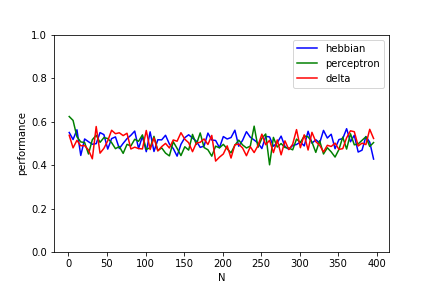
\includegraphics[width = 1.0\linewidth, trim={10 5 40 30}, clip=true]{figures/compare_prod.png}
		%\subcaption{Reference}
		%\label{}	
	\end{subfigure}%
\caption{Performance in the product-classification task as a function of the number of training vectors N for the Hebbian, perceptron and delta learning rules.}
\label{fig:performance_prod}
\end{figure}

In this case we see that all three learning rules lead to poor near-random performance.
To understand why the parity problem is so much harder than the sum problem, we again turn to the concept of linear separability. If a problem is linearly separable, there exists a (hyper)plane that can succesfully separate all possible inputs into the two output categories. In this case, it is guaranteed that the perceptron learning rule will lead to perfect performance on the training data if trained for long enough.
The sum problem is indeed linearly separable; a feature that is illustrated in two dimensions in figure \ref{fig:sum2d}. Here, the axes indicate the values of the two input elements, and the color of the dots indicate whether they should be classified as +1 (blue) or -1 (red). For the sum problem, the 0-sum vectors are undefined, but we see that they can easily be included in either category and we can still draw a single line that separates the blue (and green) dots from the red dots. This defines linear separability in two dimensions.

\begin{figure}[h]
	\centering
	\begin{subfigure}[t]{0.36\linewidth}
		\centering
		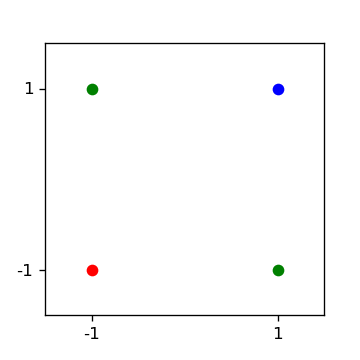
\includegraphics[width = 1.0\linewidth, trim={0 0 0 0}, clip=true]{figures/sum_2d.png}
		\subcaption{Sum problem}
		\label{fig:sum2d}	
	\end{subfigure}%
	\hspace{0.05 \linewidth}
	\begin{subfigure}[t]{0.36\linewidth}
		\centering
		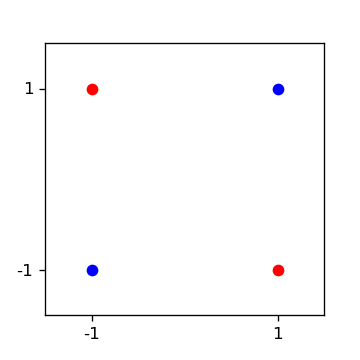
\includegraphics[width = 1.0\linewidth, trim={0 0 0 0}, clip=true]{figures/prod_2d.png}
		\subcaption{Parity problem}	
		\label{fig:prod2d}
	\end{subfigure}%
\caption{Illustration in two dimensions of the linear separablility of the sum problem and the lack thereof in the parity problem. Axes indicate elements of the two-dimensional input vector, dot color indicates the desired classification as +1 (blue), -1 (red) or undefined (green) as a function of the input elements.}
\label{fig:2dproj}
\end{figure}

\newpage

From figure \ref{fig:prod2d} on the other hand, we see that the parity problem is not linearly separable as we cannot draw a line that separates the red from the blue dots. The best we can achieve here is a 75\% succes rate by erroneously including one red dot with the blue dots or vice versa. This linear inseparability generalizes to higher dimensions and explains why the perceptron cannot solve the parity problem.
In such non-separable cases, we instead need multi-layer perceptrons which can succesfully transform the non-separable problem into a separable problem and then solve it. This is the topic of the next section.

\newpage













\section{Multi-layer perceptron}

To construct a multilayer perceptron, we first relax the constraint that inputs and outputs must be binary. We then add a single hidden layer to give the fully connected network in figure \ref{fig:network} where the dimensionalities are given for the MNIST problem. In the following, we subscript the input, hidden and output layers with $i, j, k$ respectively.

\begin{figure}[h]
	\centering
	\begin{subfigure}[t]{0.32\linewidth}
		\centering
		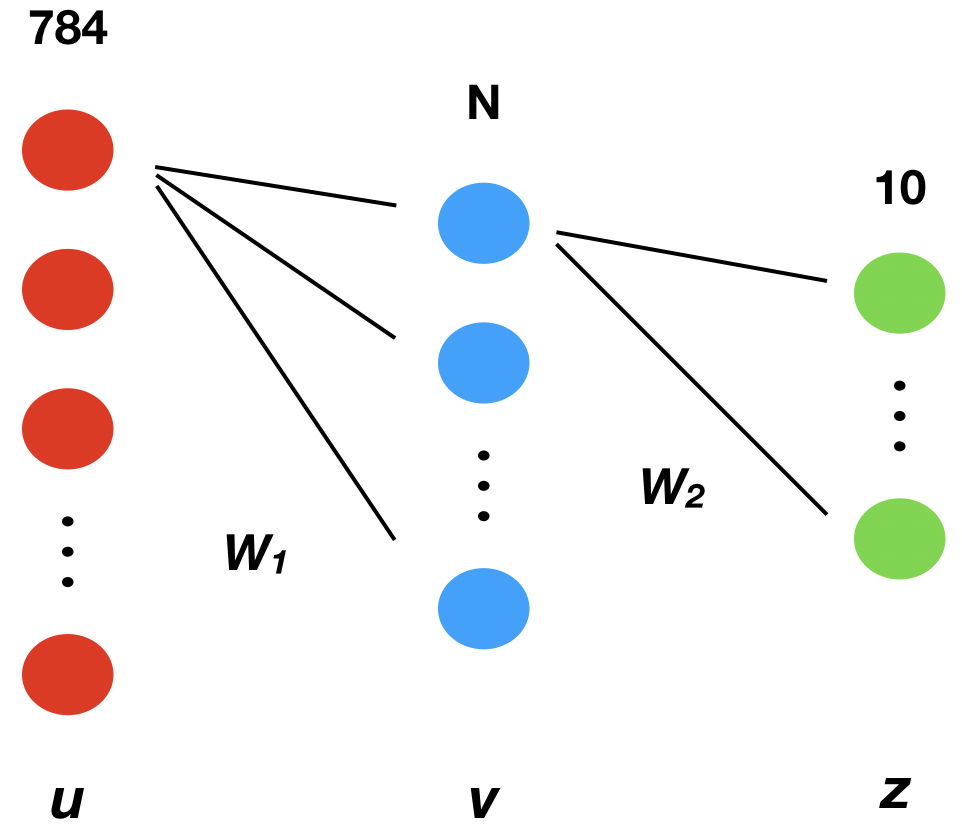
\includegraphics[width = 1.0\linewidth, trim={0 0 0 0}, clip=true]{figures/network_structure.png}
		%\subcaption{Reference}
		%\label{}	
	\end{subfigure}%
\caption{Illustration of the multi-layer perceptron as a fully connected network. Labels above nodes indicate dimensionalities for the MNIST problem, labels below nodes indicate the notation used in the present report.}
\label{fig:network}
\end{figure}

To implement the multi-layer perceptron, we need a differentiable transfer function and initially choose the tanh function $f(x) = \dfrac{e^x-e^{-x}}{e^x+e^{-x}}$ for consistency with the above step function in the single perceptron, which corresponds to the tanh function in the limit of infinite scaling. We will also consider the sigmoidal function $f(x) = \dfrac{1}{1+e^x}$ later in the report.

Denoting the activities of the input, hidden and output layers ${\bf u}, {\bf v}, {\bf z}$ respectively, we have
\begin{equation}
{\bf v} = f( {\bf u W_1} )
\end{equation}
\begin{equation}\label{eq:layer2}
{\bf z} = f( {\bf v W_2} )
\end{equation}
Here $\bf{W}_1$ is a 784xN matrix and $\bf{W}_2$ is an Nx10 matrix for the MNIST problem, and $f$ denotes element-wise application of our transfer function.

In order to train the network, we first define an error function
\begin{equation}
E = \dfrac{1}{2} \sum_k{(t_k - z_k)}
\end{equation}
Here, $t_k$ is a 1-hot representation of the training signal for input $k$. We then minimize this error using backpropagation. This corresponds to implementing a learning rule where 
\begin{equation}
\Delta w_{ij} = - \eta \dfrac{\partial E}{\partial w_{ij}}
\end{equation}

For the second set of weights ${\bf W}_2$, we can easily calculate the required derivative using the chain rule and equation \ref{eq:layer2}
\begin{equation}
\dfrac{\partial E}{\partial w_{jk}} = -(t_k - z_k)\dfrac{\partial z_k}{\partial w_{jk}} = -(t_k - z_k)f'(\sum_j{w_{jk}v_j})v_j
\end{equation}
For the tanh function, $f'(x) = 1- f(x)^2$, and we can thus use the activities computed in the forward pass to also calculate the weight changes in our backpropagation step since this implies $f'(\sum_j{w_{jk}v_j}) = 1 - z_k^2$ (for the sigmoidal transfer function, $f'(x) = f(x)-f(x)^2$ instead).
Defining $\delta_{k} = (t_k - z_k)(1-z_k ^ 2)$ for the tanh transfer function, this gives our second layer learning rule as
\begin{equation}
\Delta w_{jk} = \eta \delta_{k} v_j
\end{equation}

For the first layer of weights ${\bf W}_1$, we need to apply the chain rule repeatedly and arrive at
\begin{equation}
\dfrac{\partial E}{\partial w_{ij}} = - u_i f'(\sum_j{w_{ij}u_i}) \sum_k{[(t_k - z_k)f'(\sum_j{w_{jk}v_j})w_{jk}]}
\end{equation}
Using the fact that $f'(\sum_j{w_{ij}u_i}) = 1 - v_j^2$ for the tanh transfer function, this gives
\begin{equation}
\dfrac{\partial E}{\partial w_{ij}} = - u_i (1 - v_j^2) \sum_k{[(t_k - z_k)(1 - z_k^2)w_{jk}]}
\end{equation}
Inserting the above definition of $\delta k$ we can further define
\begin{equation}
\delta_j = (1- v_j^2) \sum_k{\delta_k w_{jk}}
\end{equation}
This finally gives an update rule for our first layer of weights
\begin{equation}
\Delta w_{ij} = \eta \delta_{j} u_i
\end{equation}

We first validate our implementation of the MLP on the parity problem from the single perceptron section. We train the system on 400 training inputs and quantify its classification success on 1000 randomly generated queries as above. For this preliminary analysis, we fix our learning rate at $\eta = 0.05$ and $N = 50$ and include bias units. Defining an epoch as a single pass of elementwise training on the full training dataset, we plot the classification performance as a function of epoch number in figure \ref{fig:mlp_parity}.

\begin{figure}[h]
	\centering
		\begin{subfigure}[t]{0.42\linewidth}
		\centering
		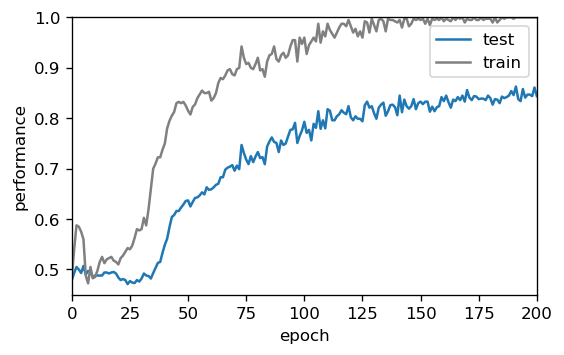
\includegraphics[width = 1.0\linewidth, trim={5 5 5 5}, clip=true]{figures/N50_eta05_nepoch200_transfer_tanh_parity_performance.png}
		\subcaption{}	
		%\label{}
	\end{subfigure}%
	\hspace{0.05 \linewidth}
	\begin{subfigure}[t]{0.42\linewidth}
		\centering
		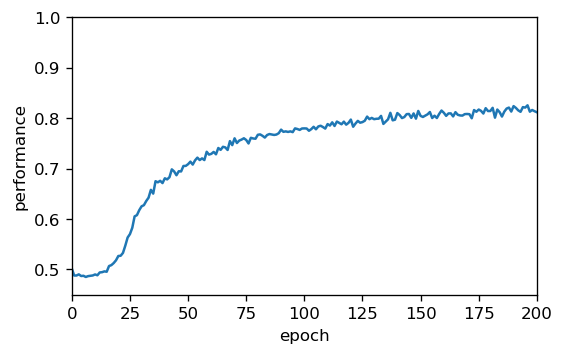
\includegraphics[width = 1.0\linewidth, trim={5 5 5 5}, clip=true]{figures/N50_eta075_nepoch200_ntrial10_transfer_tanh_parity_performance.png}
		\subcaption{}
		%\label{}	
	\end{subfigure}%
\caption{Performance of a multi-layer perceptron with $N=50$ and $\eta = 0.05$ in the parity problem. (a) Performance in a single trial for both the test and training data, (b) mean test performance over 10 independent trials.}
\label{fig:mlp_parity}
\end{figure}

%\newpage

We see that the multi-layer perceptron succesfully learns the problem to an accuracy of just over 80\%, while the performance on the training data goes to 100\%. This shows that our implementation does indeed work and that a multi-layer perceptron can solve the parity problem. We will discuss the use of dropout to diminish the training-test performance gap later.

Having validated our MLP, we move on to the MNIST dataset consisting of 60,000 handwritten training digits and 10,000 test digits. We provide the input data as 784-element vectors rescaled such that all elements are between 0 and 1. Our labels are provided as 10-element 1-hot representations of the correct digit.
Running a first-pass training with $N=50$ and $\eta = 0.05$ similar to above, we see that the multi-layer perceptron can also learn the MNIST problem without much parameter optimization (figure \ref{fig:N50})

\begin{figure}[h]
	\centering
	\begin{subfigure}[t]{0.42\linewidth}
		\centering
		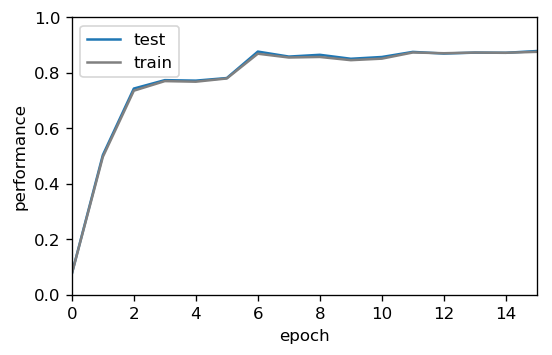
\includegraphics[width = 1.0\linewidth, trim={5 5 5 5}, clip=true]{figures/N50_eta05_nepoch15_transfer_tanh_performance.png}
		\subcaption{}
		%\label{}	
	\end{subfigure}%
	\hspace{0.05 \linewidth}
	\begin{subfigure}[t]{0.42\linewidth}
		\centering
		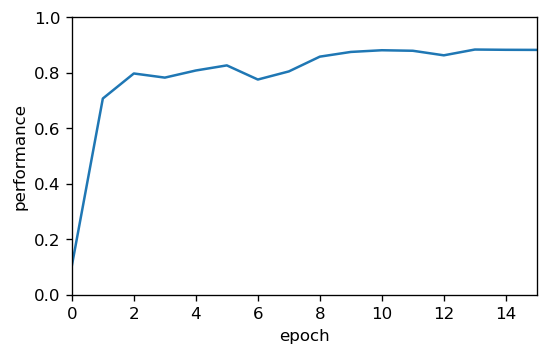
\includegraphics[width = 1.0\linewidth, trim={5 5 5 5}, clip=true]{figures/N50_eta05_nepoch15_ntrial5_transfer_tanh_performance.png}
		\subcaption{}	
		%\label{}
	\end{subfigure}%
\caption{Performance of a multi-layer perceptron with $N=50$ and $\eta = 0.05$ in the MNIST problem. (a) Test and training performance in a single trial, (b) mean test performance over 5 independent trials.}
\label{fig:N50}
\end{figure}

\newpage

For this analysis, the pythin implementation took an average of 150 seconds per epoch, making an extensive parameter search and optimization challlenging. However, converting the same algorithm to julia lead to a 50-fold improvement in computation time to 3.1 seconds per epoch, allowing us to investigate more thoroughly the effect of various network parameters on the performance of the network (note that all training is carried out with a batch size of 1 leading to relatively long epochs).

We start by investigating the effect of the number of hidden units N and the learning rate $\eta$ in a simple network with no bias units. We carry out an exhaustive search for small N with the result given in figure \ref{fig:scan_N_eta}.

\begin{figure}[h]
	\centering
	\begin{subfigure}[t]{0.42\linewidth}
		\centering
		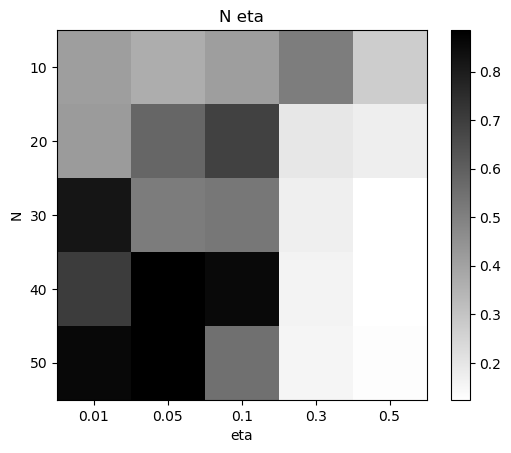
\includegraphics[width = 1.0\linewidth, trim={0 0 0 0}, clip=true]{figures/scan_N_eta_perf.png}
		%\subcaption{Performance on the test data}
		%\label{}	
	\end{subfigure}%
	\hspace{0.05 \linewidth}
	\begin{subfigure}[t]{0.42\linewidth}
		\centering
		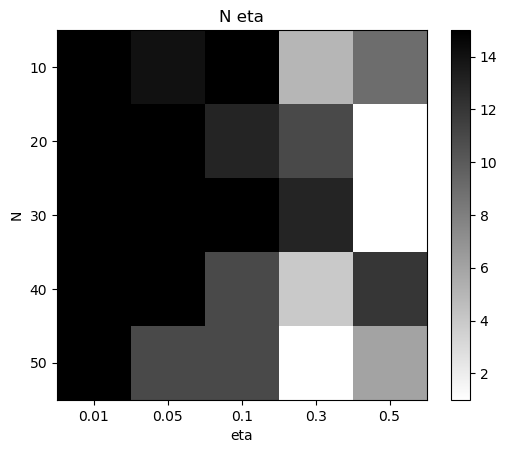
\includegraphics[width = 1.0\linewidth, trim={0 0 0 0}, clip=true]{figures/scan_N_eta_epochs.png}
		%\subcaption{number of epochs to reach maximum performance capped at 15}	
		%\label{}
	\end{subfigure}%
\caption{\textit{left}: maximum classification performance as a function of N and $\eta$. \textit{right}: number of epochs after which the maximum performance is observed. The training sessions were capped at 15 epochs. Performances were averaged over 5 independent networks.}
\label{fig:scan_N_eta}
\end{figure}

We firstly note that an average performance of almost 90\% is achieved for a range of different parameters, indicating that even a very simple and relatively small network can achieve a decent performance in the MNIST classification problem. We also note that the optimum performance is generally achieved after 15 epochs, suggesting that further training can lead to additional improvements. Finally, we see that as the network size increases, we require a smaller learning rate to achieve optimum performance. This is because an increased network size will otherwise lead to a very large total change in weights per epoch.

From figure \ref{fig:scan_N_eta} we also see that we achieve good performance for a relatively small network with N=50 and $\eta = 0.01$. We therefore use these parameter values to generate learning curves for fixed N and variable $\eta$ and vice versa in figure \ref{fig:learning_curves} to get a better understanding of the effect of these parameters on our network.

\begin{figure}[h]
	\centering
	\begin{subfigure}[t]{0.42\linewidth}
		\centering
		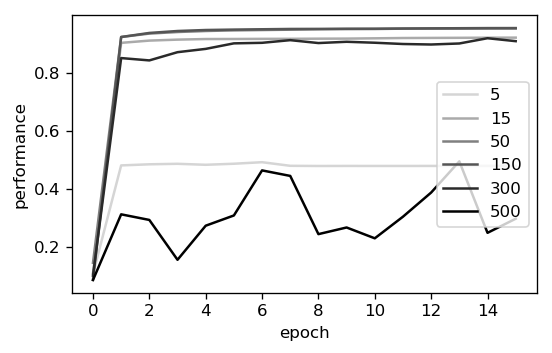
\includegraphics[width = 1.0\linewidth, trim={5 5 5 5}, clip=true]{figures/test_N_bigrange.png}
	\end{subfigure}%
	\hspace{0.05 \linewidth}
	\begin{subfigure}[t]{0.42\linewidth}
		\centering
		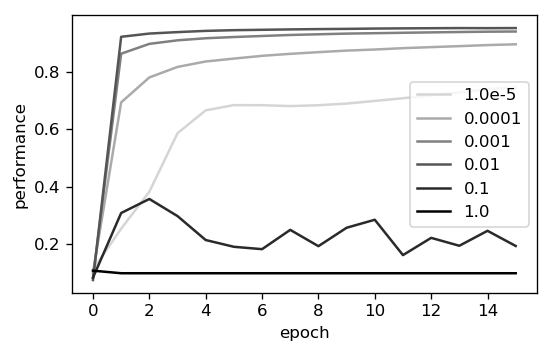
\includegraphics[width = 1.0\linewidth, trim={5 5 5 5}, clip=true]{figures/testeta_real.png}
	\end{subfigure}%
\caption{Learning curves for variable N (left) and $\eta$ (right) with the reciprocal parameter fixed at $\eta=0.01$ and N=50 respectively. Variable parameters are given in the legends with darker lines corresponding to higher parameter values. Performances are averaged over 3 trials.}
\label{fig:learning_curves}
\end{figure}

\newpage

We see that as N increases, the converged performance initially increases followed by a plateau of similar performance for N=15-300 (note that the N=50 and N=150 curves coincide). Finally, performance drops catastrophically when the network size becomes too large compared to our learning rate. Together with figure \ref{fig:scan_N_eta} this suggests that increased network size leads to improved performance provided the learning rate has been optimized.

When our learning rate increases, we similarly observe an initial increase in converged performance for a range of $\eta$ as well as an increase in the rate of learning. However, once $\eta$ becomes too high compared to N, we observe a catastrophic decrease in performance as the network jumps around the energy landscape rather than descending monotonously.

Taken together, these observations suggest that we can improve performance by increasing network size, but this requires individual optimizations of the learning rates for different network sizes and also leads to increased computational costs since larger networks have more parameters and also require smaller learning rates and thus exhibit slower learning. Additionally, we expect that if the networks become large enough relative to our training data, we will observe overfitting and a decrease in test performance. Given the present computational and algorithmic limitations, this has not been observed.

Based on these investigations, it is clear that we can achieve sensible performances with no bias units, but we now proceed to investigate the effect of bias units for the input and hidden layers. Bias units are additional nodes with a constant value of 1, fully connected to the next downstream layer. These nodes allow us to shift the function we are fitting and thus learn more complex datasets. We therefore expect the addition of bias nodes to improve performance, and indeed it is somewhat surprising that we are able to learn the MNIST dataset with no bias nodes in the first place.

Surprisingly therefore, it turns out that adding bias nodes does not lead to an observable performance increase for our network with N=50 and $\eta=0.01$ (figure \ref{fig:biastanh}). One possibility is that this lack of effect is due to us using an antisymmetric transfer function under the hypothesis that in the case where $f(x = 0) \neq 0$, shifting the fitted function becomes more important. We therefore modify our MLP to be able to use the sigmoidal transfer function, but still do not observe a difference between networks with and without bias units (figure \ref{fig:biassigmoid}). Finally, we investigate whether the lack of effect is due to the particular representation of the data that we use such that shifting the input data might necessitate bias units. We therefore shift all input vectors by 0.625 and train the network on this new input dataset (figure \ref{fig:biasshifted}).

\begin{figure}[h]
	\centering
	\begin{subfigure}[t]{0.32\linewidth}
		\centering
		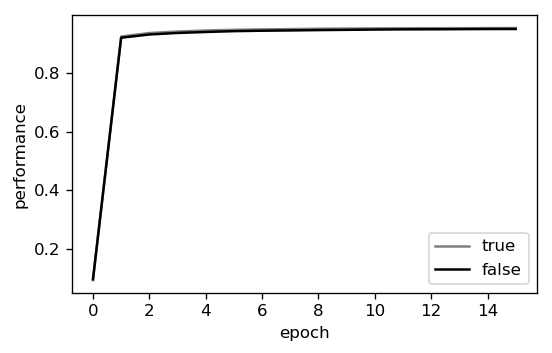
\includegraphics[width = 1.0\linewidth, trim={5 5 5 5}, clip=true]{figures/bias_tanh.png}
		\subcaption{}
		\label{fig:biastanh}	
	\end{subfigure}%
	\hspace{0.01 \linewidth}
	\begin{subfigure}[t]{0.32\linewidth}
		\centering
		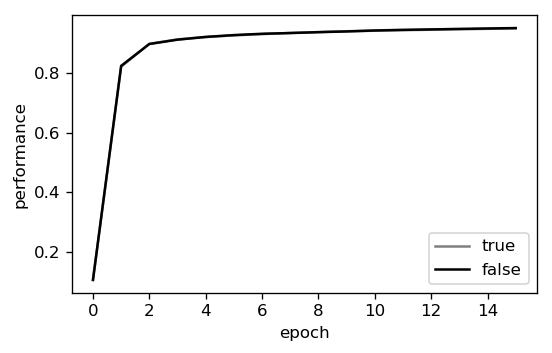
\includegraphics[width = 1.0\linewidth, trim={5 5 5 5}, clip=true]{figures/test_bias_sigmoid.png}
		\subcaption{}	
		\label{fig:biassigmoid}
	\end{subfigure}%
	\hspace{0.01 \linewidth}
	\begin{subfigure}[t]{0.32\linewidth}
		\centering
		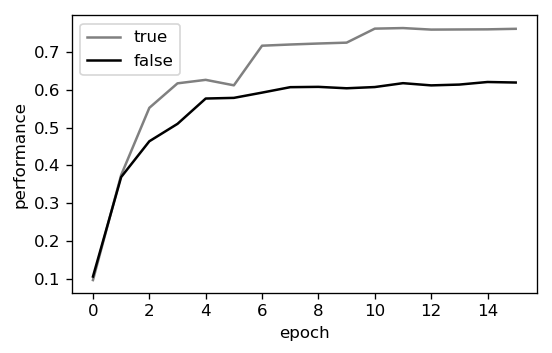
\includegraphics[width = 1.0\linewidth, trim={5 5 5 5}, clip=true]{figures/test_bias_shift725.png}
		\subcaption{}	
		\label{fig:biasshifted}
	\end{subfigure}%
\caption{Performance of the MLP on the MNIST dataset with (grey) and without (black) bias units. (a) performance in the simple case, (b)  performance with a sigmoidal transfer function (c) performance after shifting the input data by 0.625.}
\label{fig:biasunits_tanh}
\end{figure}

\newpage


We see that the inclusion of bias units does indeed lead to improved performance for this shifted dataset, indicating that the importance of bias units depends on the particular input dataset in question. To investigate this further, we therefore run a similar comparison on the parity problem and see that there is a very large difference in performance between networks with and without bias units for this particular problem (figure \ref{fig:bias_parity}).

\begin{figure}[h]
	\centering
	\begin{subfigure}[t]{0.42\linewidth}
		\centering
		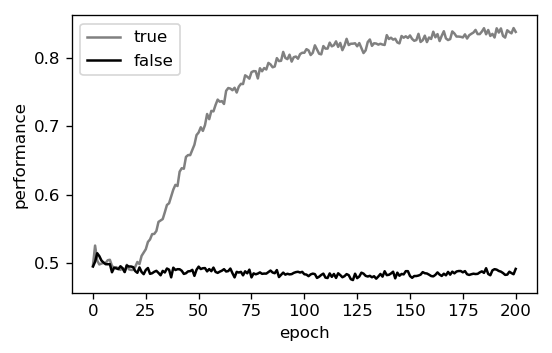
\includegraphics[width = 1.0\linewidth, trim={0 0 0 0}, clip=true]{figures/bias_parity.png}
		%\subcaption{}
		%\label{fig:biastanh}	
	\end{subfigure}%
	\hspace{0.02 \linewidth}
	\begin{subfigure}[t]{0.42\linewidth}
		\centering
		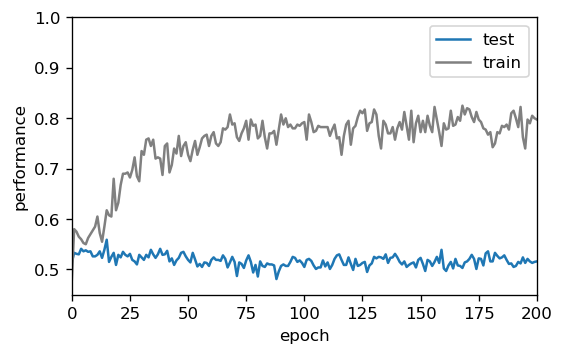
\includegraphics[width = 1.0\linewidth, trim={0 0 0 0}, clip=true]{figures/nobias_N50_eta05_nepoch200_transfer_tanh_parity_performance.png}
		%\subcaption{}
		%\label{fig:biastanh}	
	\end{subfigure}%
\caption{Importance of bias units for the parity problem. (a) mean performance with (grey) and without (black) bias units on the test data over 10 trials. (b) performance on the test (blue) and train (grey) data for a single trial with no bias units. N=50 and $\eta = 0.05$ for both plots.}
\label{fig:bias_parity}
\end{figure}

%\newpage

In this case, the network completely fails to solve the parity problem in the absence of bias units, with the asymptotic performance being even worse than random guessing. On the contrary, the network with bias units learns the problem with an asymptotic test performance greater than 80\%. We thus conclude that bias units can greatly improve performance for certain types of input, while it is relatively unnecessary if the data has been appropriately preprocessed. However, in general the inclusion of bias units does lead to improved performance with little increase in computational cost, and we therefore include them for all subsequent analyses.

 We also see from figure \ref{fig:biassigmoid} that the performance with the sigmoidal transfer function is very similar to what we observed for the tanh transfer function and therefore provide a direct comparison in figure \ref{fig:transfers} showing that the asymptotic performance is indeed similar although the tanh network learns more quickly.

\begin{figure}[h]
	\centering
	\begin{subfigure}[t]{0.52\linewidth}
		\centering
		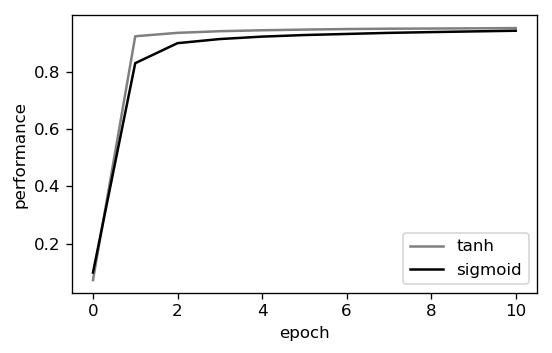
\includegraphics[width = 1.0\linewidth, trim={5 5 5 5}, clip=true]{figures/tanh_sigmoidal_transfers.png}
		%\subcaption{}
		%\label{fig:biastanh}	
	\end{subfigure}%
\caption{Performance with tanh (grey) and sigmoidal (black) transfer functions for a network with N=50, $\eta = 0.01$, including bias units, and averaged over 3 trials.}
\label{fig:transfers}
\end{figure}

\newpage

Although we have predominantly investigated small network above, we note that LeCun et al. (1998) achieved MNIST error rates of 4.7\% and 4.5\% with 300 and 1000 hidden units respectively. For the purpose of investigating the classification efficiency of the MLP on the MNIST data, we therefore train a new network with 300 nodes for 20 epochs with a learning rate of 0.005 (optimization not shown) after which the performance has reached 96.2\% (figure \ref{fig:N300_performance}). This corresponds to an error rate of 3.8\% and is thus better than both LeCun's 300-node and 1000-node networks.

\begin{figure}[h]
	\centering
	\begin{subfigure}[t]{0.52\linewidth}
		\centering
		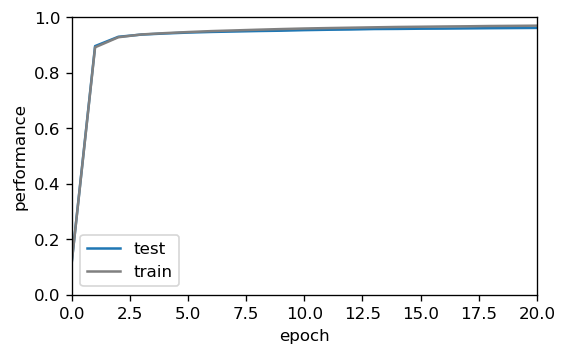
\includegraphics[width = 1.0\linewidth, trim={5 5 5 5}, clip=true]{figures/bias_N300_eta005_nepoch20_transfer_tanh_performance.png}
		%\subcaption{}
		%\label{fig:biastanh}	
	\end{subfigure}%
\caption{Learning curve for a network with 300 hidden nodes and $\eta=0.005$. Note that even for this larger network, we do not overfit the data.}
\label{fig:N300_performance}
\end{figure}

%\newpage

After training the network, we can look at the types of errors it makes to see if there are any particular classifications it struggles with.  We therefore plot a histogram of the performance for the 10 different digits in figure \ref{fig:predictionhist} and see that the performance for different digits does vary significantly. Notably, performance is very low for '2' and '5' while it is very high for '0' and '1'.
To understand why this is the case, we further plot a cross-prediction matrix in figure \ref{fig:predictions}. This shows for each target digit (rows) how often the network classifies this digit as each of the 10 digits (columns).

\begin{figure}[h]
	\centering
	\begin{subfigure}[t]{0.48\linewidth}
		\centering
		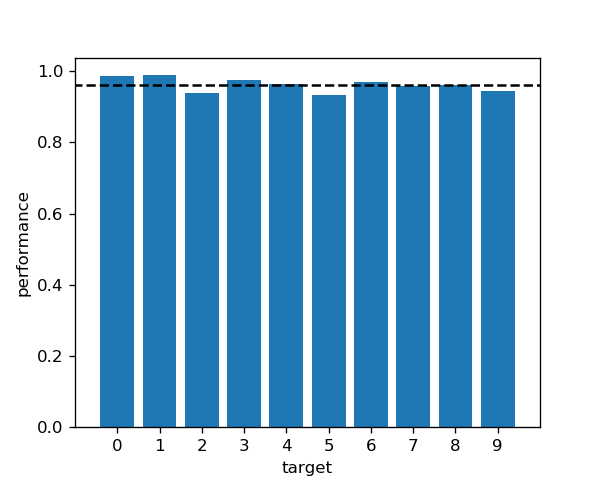
\includegraphics[width = 1.0\linewidth, trim={0 0 0 0}, clip=true]{figures/predictionhist.png}
		\subcaption{}
		\label{fig:predictionhist}	
	\end{subfigure}%
	\hspace{0.02 \linewidth}
	\begin{subfigure}[t]{0.42\linewidth}
		\centering
		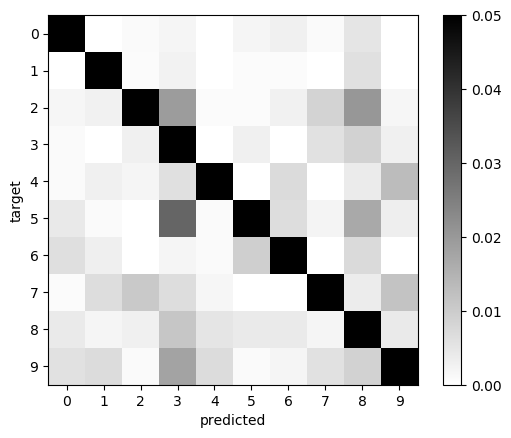
\includegraphics[width = 1.0\linewidth, trim={0 0 0 0}, clip=true]{figures/predictions.png}
		\subcaption{}
		\label{fig:predictions}	
	\end{subfigure}%
\caption{(a) Performance for each of the 10 digits. Dashed line indicates mean performance across test data. (b) Cross-prediction showing how often a given number is predicted for each correct digit. Note that the colormap is capped at 0.05 so we cannot resolve the diagonal elements. However, these values are given in figure (a), and the low cap allows us to better distinguish the off-diagonal elements. }
\label{fig:prediction_errors}
\end{figure}

\newpage

Notably, '2' and '5' are both commonly confused as '3' and '8' but not vice versa, leading to the poor performance for these digits observed in figure \ref{fig:predictionhist}. In general, we see that many other digits are commonly misclassified as '3' and '8'. This suggests that these two digits are polymorphic in the training data and the corresponding classes therefore occupy a large volume of input parameter space.
These observations are similar to what we see using a sigmoidal transfer function (figure \ref{fig:prediction_error_sigmoid}) or different N and $\eta$ (not shown), suggesting that they are features of the data rather than the particular network instance.

\begin{figure}[h]
	\centering
	\begin{subfigure}[t]{0.48\linewidth}
		\centering
		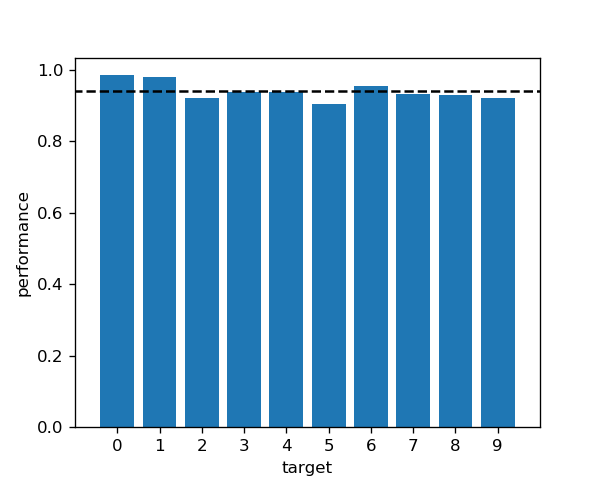
\includegraphics[width = 1.0\linewidth, trim={0 0 0 0}, clip=true]{figures/predictionhist_sigmoid.png}
		\subcaption{}
		\label{fig:predictionhist_sigmoid}	
	\end{subfigure}%
	\hspace{0.02 \linewidth}
	\begin{subfigure}[t]{0.42\linewidth}
		\centering
		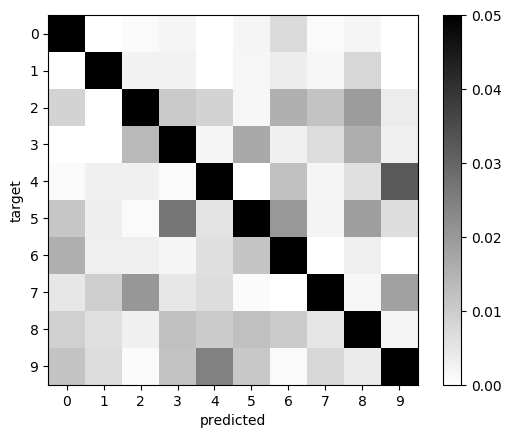
\includegraphics[width = 1.0\linewidth, trim={0 0 0 0}, clip=true]{figures/predictions_sigmoid.png}
		\subcaption{}
		\label{fig:predictions_sigmoid}	
	\end{subfigure}%
\caption{(a) Performance for each of the 10 digits with a sigmoidal transfer function. (b) Cross-prediction showing how often a given number is predicted for each correct digit.}
\label{fig:prediction_error_sigmoid}
\end{figure}

\newpage

To understand how the network manages to correctly identify the digits, we train a network with 10 hidden units for 20 epochs, achieving a performance of 90.8\%. We then plot in figure \ref{fig:w1s_N10} for each hidden unit the weights from the input layer to that unit, reshaped to correspond to the input images. This shows the features that lead to activation of each of the input units.

\begin{figure}[h]
	\centering
	\begin{subfigure}[t]{0.92\linewidth}
		\centering
		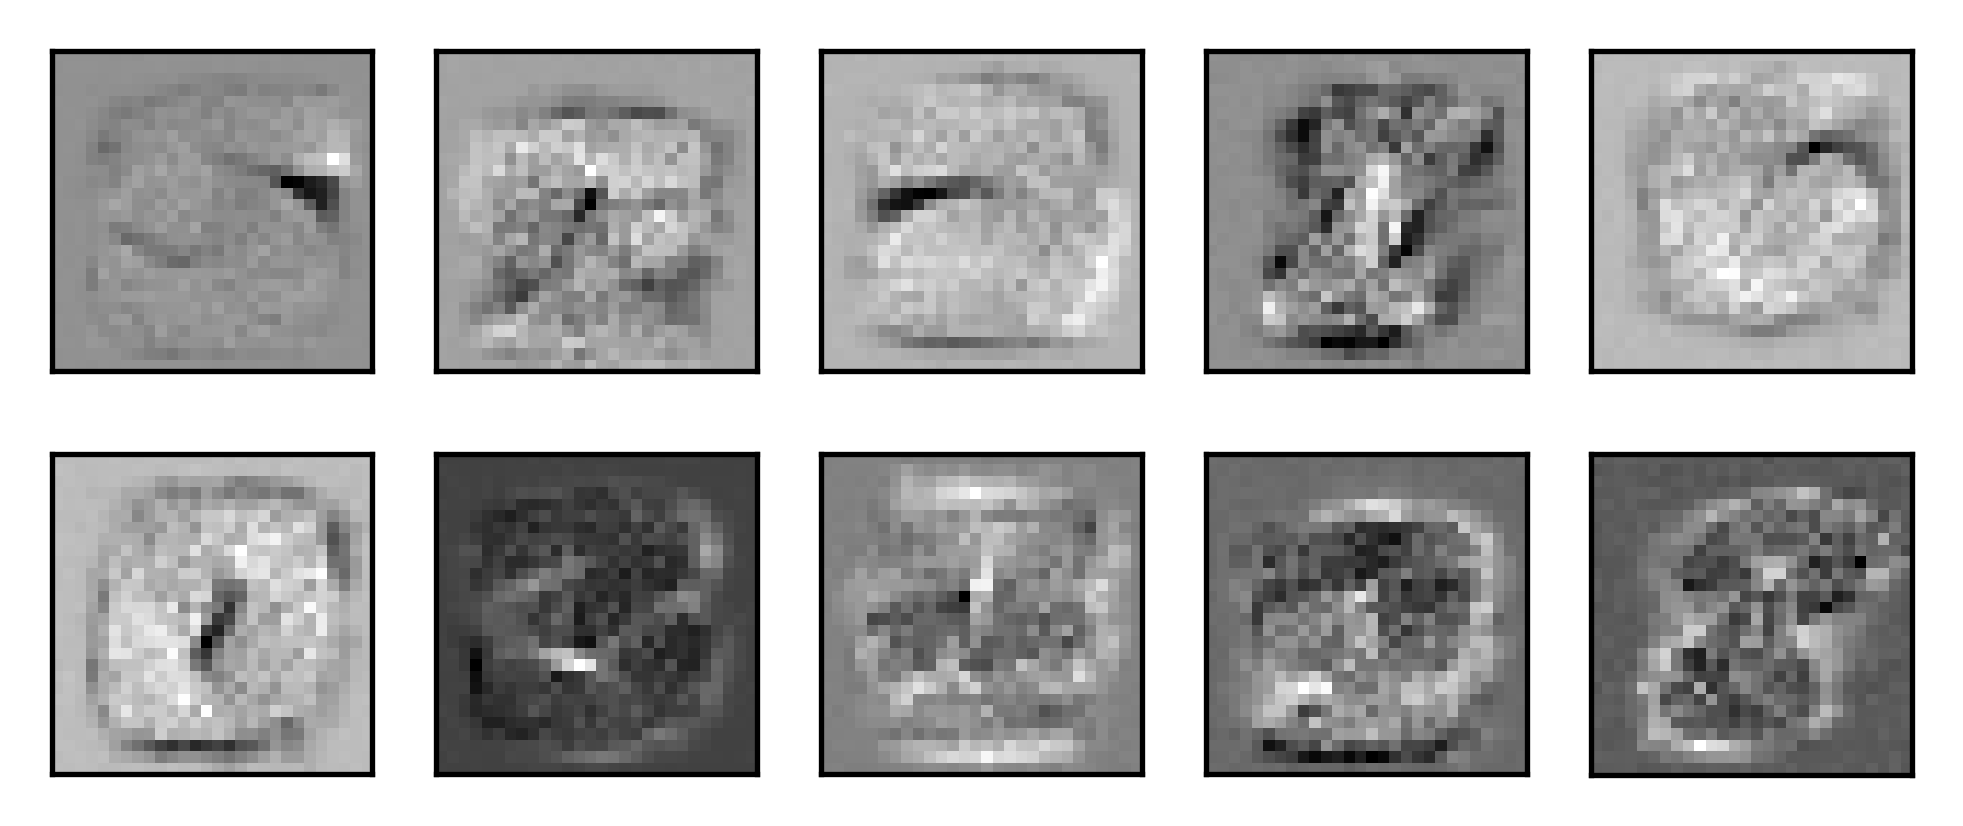
\includegraphics[width = 1.0\linewidth, trim={0 0 0 0}, clip=true]{figures/w1s_N10_weightfig.png}	
	\end{subfigure}%
\caption{Input weights for each hidden unit in a 10-unit network, reshaped to resemble the input images before flattening.}
\label{fig:w1s_N10}
\end{figure}

We see that in the case of N=10, there are recognizable patterns already in the hidden layer which e.g. contains nodes resembling the numbers 0 and 3 (bottom left). Since many weights and all activations are less than 0, much of the network operates in the linear regime of the tanh function, and we can therefore get an idea of the activation of the output layer by multiplying the ${\bf W}_1$ and ${\bf W}_2$ matrices. We plot the resulting pseudoweights from the input layer to the output layer in figure \ref{fig:w3s_N10}

\begin{figure}[h]
	\centering
	\begin{subfigure}[t]{0.92\linewidth}
		\centering
		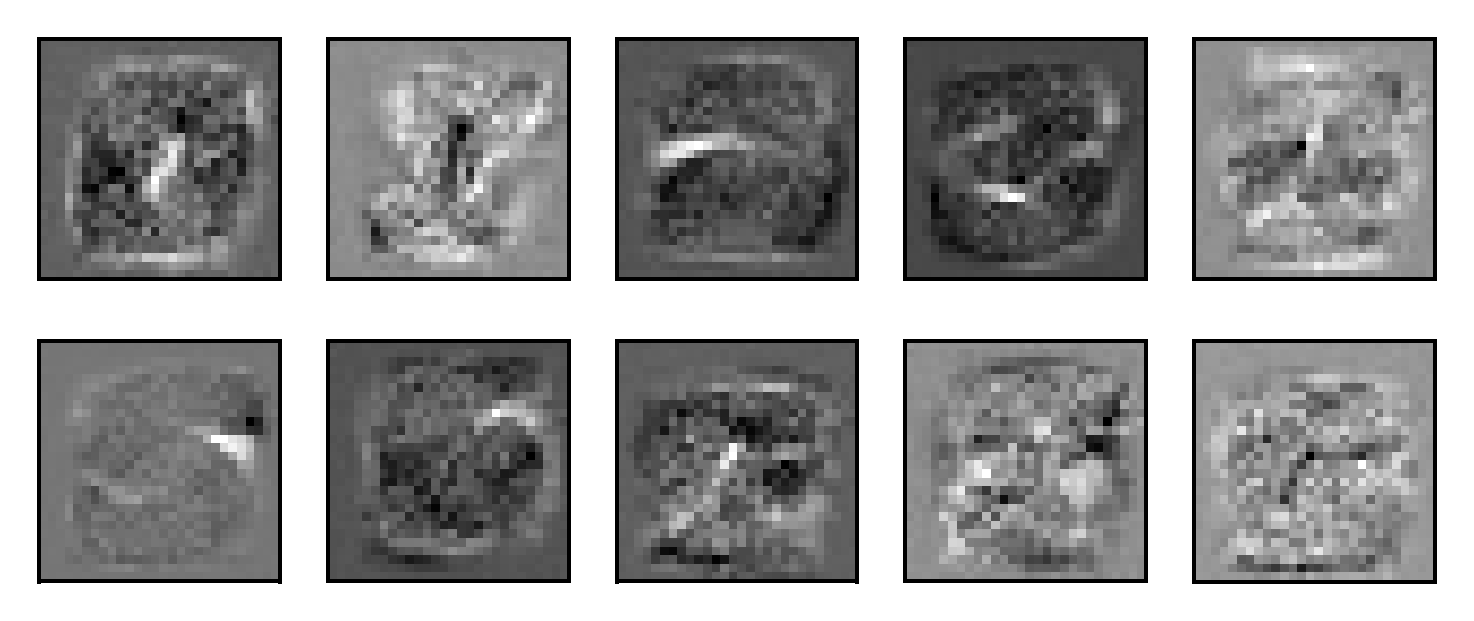
\includegraphics[width = 1.0\linewidth, trim={0 0 0 0}, clip=true]{figures/w3s_N10_weightfig.png}
	\end{subfigure}%
\caption{Rowplot of ${\bf W}_1 \cdot {\bf W}_2$ in a 10-unit network, reshaped to resemble the input images before flattening.}
\label{fig:w3s_N10}
\end{figure}

%\newpage

We see that some of these units resemble those in the hidden layer, and a manual inspection of the weights confirms that these have a single dominant input from the hidden layer. Other output units are combinations of hidden units with e.g. output unit 5 corresponding to the number '4' having coefficients of -0.8 from both the first and tenth hidden units and near-zero weights from all other hidden units. In general, we see that most of the activations resemble the digits we are trying to predict with exceptions including '8' - a digit we already know to be rather 'diffuse' in input space from our cross-prediction matrix above.

For larger network sizes, the output units are increasingly made up of combinations of hidden units which are used as a basis for classification to leverage the increased dimensionality of parameter space. This is also expected since we would otherwise achieve comparable performance with single-layer networks.
Rather than observing hidden units with activations resembling actual digits, we therefore also see that the activations can now resemble 'features' such as circles or edges. As an example, the first 10 hidden units of a trained network with N=300 have been plotted in figure \ref{fig:w1s_N300}.

\begin{figure}[h]
	\centering
	\begin{subfigure}[t]{0.92\linewidth}
		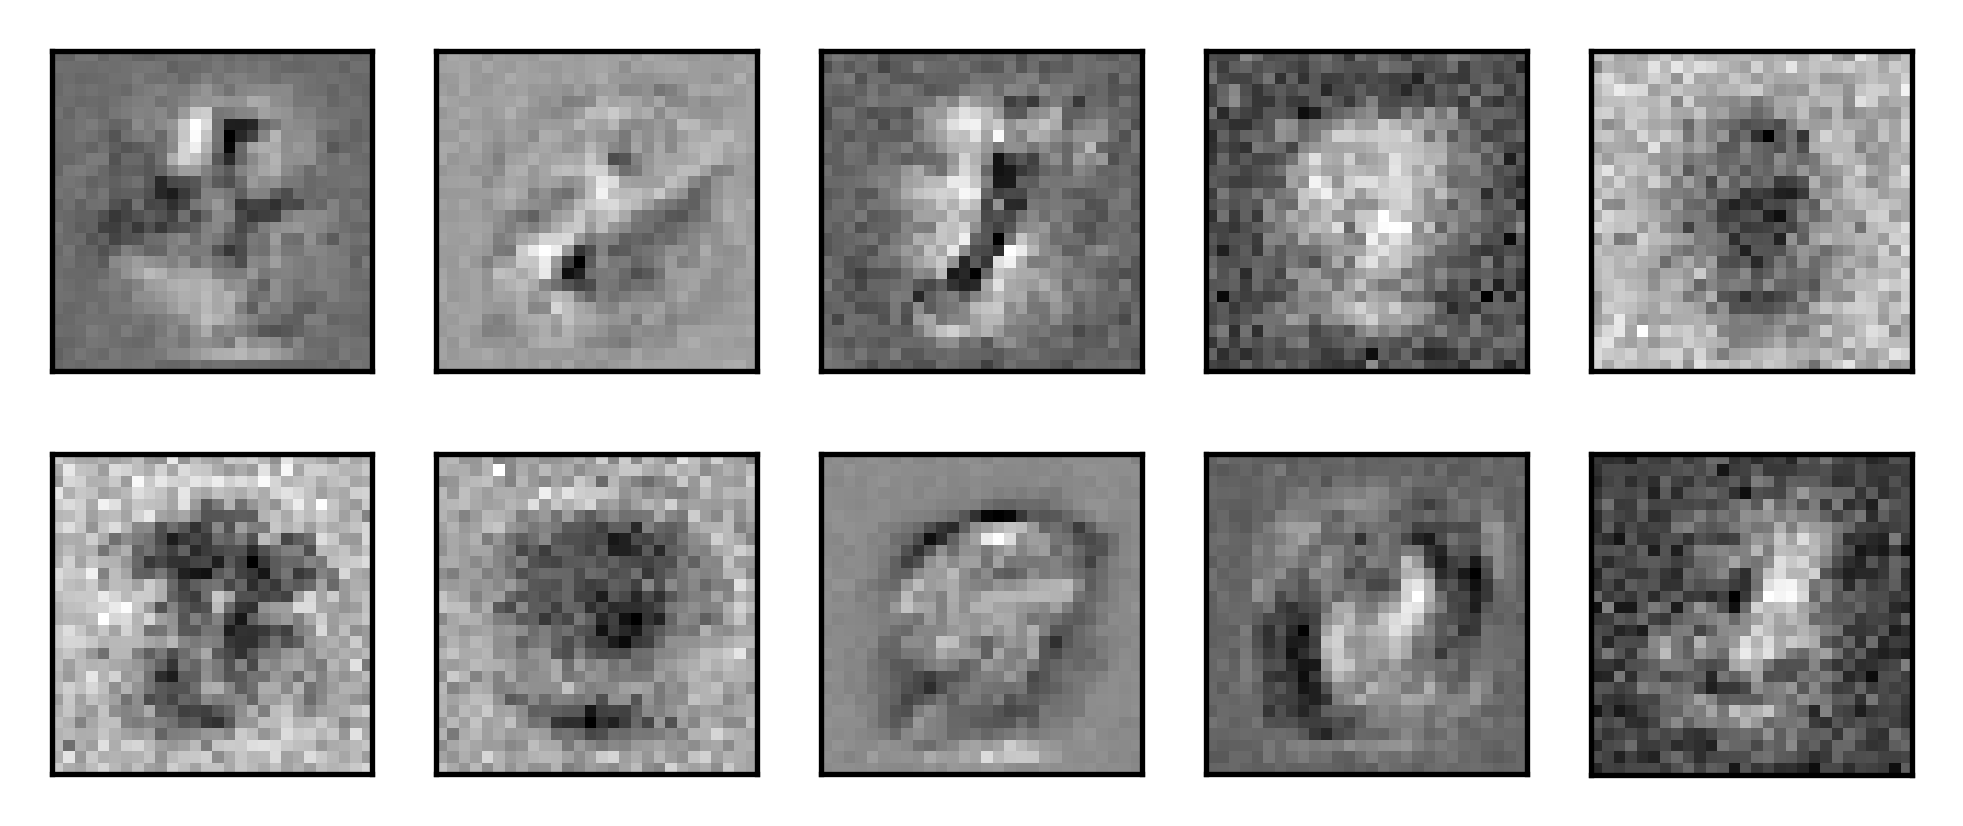
\includegraphics[width = 1.0\linewidth, trim={0 0 0 0}, clip=true]{figures/w1s_N300_weightfig.png}
	\end{subfigure}%
\caption{Input weights for each of the first 10 hidden units in a 300-unit network, reshaped to resemble the input images before flattening.}
\label{fig:w1s_N300}
\end{figure}

We thus conclude that the hidden units contribute to solving the problem in small networks by responding to one or a few digits, while the hidden units in larger networks correspond to particular features and digits are classified as particular combinations of these features by the second layer of weights.

Finally we return to the problem of overfitting, which is commonly solved using dropout as described by Srivastava et al. (2014). As we see from figure \ref{fig:N300_performance}, overfitting is not a problem in the present case of 60,000 input data points and only a few hundred hidden nodes. However, if we increase the hidden layer size to the point where overfitting might be a problem in this relatively shallow network, the computational time becomes rather overwhelming for the present implementation.

Instead of resorting to keras or pytorch, we therefore choose to downsample the original training data to investigate the effect of dropout. The downsampling of the input data serves two purposes; firstly it decreases the number of parameters we need to learn for a fixed hidden layer size, and secondly it decreases the hidden layer size needed to overfit the data. We thus achieve an approximately quadratic improvement in the time needed to investigate the effects of dropout.

We downsample the input data to just 200 digits and use 1000 random digits as our test data. We then train a network with N=1000 using a sigmoidal transfer function either with or without dropout and plot the resulting learning curves in figure \ref{fig:dropout}. In this case, we use a dropout rate of 10\% in the input layer and 40\% in the hidden layer since this was found to work well. No extensive dropout optimizations were carried out since overtraining did not occur for the full dataset, and optimizing dropout rates for the downsampled input data is therefore irrelevant for the analysis of the full network.

\begin{figure}[h]
	\centering
	\begin{subfigure}[t]{0.62\linewidth}
		\centering
		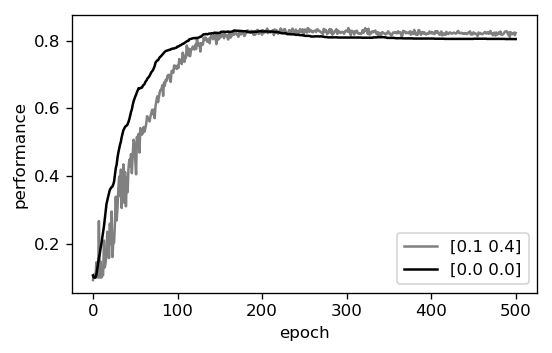
\includegraphics[width = 1.0\linewidth, trim={0 0 0 0}, clip=true]{figures/dropout_N1000_eta02.png}
		%\subcaption{}
		%\label{fig:biastanh}	
	\end{subfigure}%
\caption{Learning curves for a network with 1000 hidden nodes and $\eta=0.02$ with input data downsampled to 200 digits. Legend indicates dropout rate for the input layer and hidden layer.}
\label{fig:dropout}
\end{figure}

\newpage

We see that without dropout, training is initially faster than with dropout but peaks at a test performance of 82\% after 180 epochs following which the training performance keeps increasing while the test performance decreases to 80\% due to overfitting of the input data. This is further illustrated in figure \ref{fig:nodrop1}. When we include dropout, training is initially slower. However, the test performance continues to increase together with the training performance, and we therefore converge to a better test performance of 83\% after 500 epochs. This is further illustrated in figure \ref{fig:drop1}. On a side note, it is also rather remarkable that we can achieve 83\% efficiency with only 200 training digits.


\begin{figure}[h]
	\centering
	\begin{subfigure}[t]{0.42\linewidth}
		\centering
		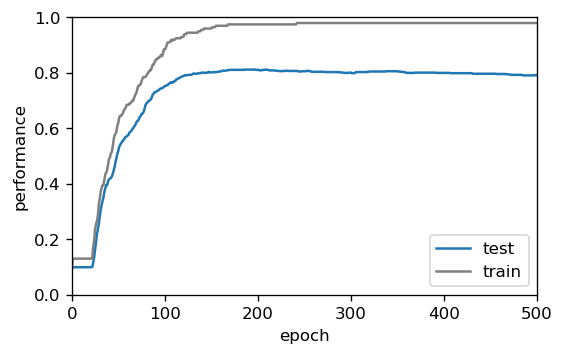
\includegraphics[width = 1.0\linewidth, trim={5 5 5 5}, clip=true]{figures/nodropout_N1000_eta02_nepoch500_transfer_sigmoid_performance.png}
		\subcaption{}
		\label{fig:nodrop1}	
	\end{subfigure}%
\hspace{ 0.02\linewidth}
	\begin{subfigure}[t]{0.42\linewidth}
		\centering
		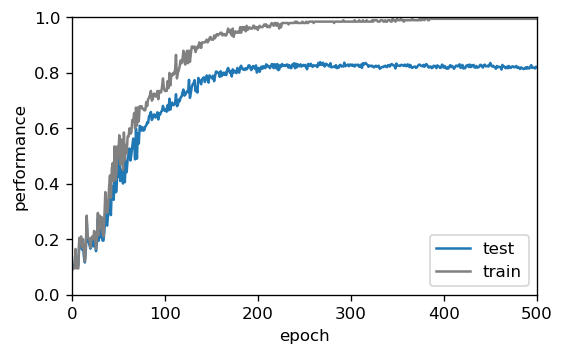
\includegraphics[width = 1.0\linewidth, trim={5 5 5 5}, clip=true]{figures/dropout_N1000_eta02_nepoch500_transfer_sigmoid_performance.png}
		\subcaption{}
		\label{fig:drop1}	
	\end{subfigure}%
\caption{Learning curves for a network with 1000 hidden nodes and $\eta=0.02$ on input data downsampled to 200 digits with (right) and without (left) dropout.}
\label{fig:dropout_test_train}
\end{figure}

%\newpage

We thus see that dropout limits overtraining by changing the combinations of weights that are trained together in each iteration. This leads to noisier and slower training but converges to a better performance when the network size is very large compared to the training dataset.
In the present case, overfitting is not very pronounced and dropout thus leads to only a modest increase in performance, but in other contexts with more compute power and larger networks, dropout or other regularization methods can be essential to train a functional network.

\newpage







\section{Critique of deep learning}

Gary Marcus, Professor of Psychology and Neural Science at New York University, published an opinion piece on arXiv in early 2018 discussing shortcomings of current approaches in deep learning and AI. The article, \textit{Deep Learning: A Critical Appraisal}, starts by assessing the current state of the field and proceeds to outline 10 limitations of deep learning. In the following, I will outline the main points and arguments made by Marcus while simultaneously commenting on his ideas using examples from the literature. I willl then outline the debate with others in the AI community that this article initiated.

In the article, Marcus sets the scene by defining deep neural networks as multi-layer networks trained by backpropagation to learn an input-output mapping in a supervised learning task, and he describes how deep learning has come to dominate the AI field since 2012. He proceeds to highlight the importance of convolutional neural networks (LeCun et al. 1989), and lists speech recognition, object recognition, and video \& board games as fields where deep learning has achieved significant advances, pointing out that with enough data and computational power, deep networks could possibly solve any desired task.
Marcus then returns to the real world of limited data and compute power which requires AI systems to generalize, and he outlines the following ten challenges faced by deep learning in this respect.
\begin{enumerate}[1]
\item \textit{Deep Learning is 'data hungry'}\\
Marcus points out that while humans are able to generalize from descriptions and a few examples using abstract relations, neural networks generally rely on large annotated datasets without the use of abstract representations. This is exemplified by the challenges faced by convolutional neural networks in generalizing to novel viewpoints in an artificial arena. However, this has since been adressed with good results by DeepMind (Eslami et al 2018) while major advances have also been made in learning from sparse data (Santoro et al. 2016). It is thus not clear that these challenges cannot be adressed by deep networks with augmented architectures.

\item \textit{Deep learning systems are conceptually shallow}\\
While the actual architectures are 'deep' (i.e. contain multiple layers), Marcus argues that neural networks have no deep understanding of the tasks at hand. This is exemplified by DeepMind's Atari system which fails when the Y-coordinate of the paddle is altered since it has not learned that the ball must hit the paddle but merely how the paddle should move depending on where the ball is. I agree with Marcus that this lack of generalization between related tasks appears to be a significant shortcoming in the field which deep learning does not have an obvious solution to.

\item \textit{Deep learning struggles to represent hierarchical structure}\\
In e.g. human language processing, we understand that there is a hierarchy to the sentences we use and hear. On the contrary, a neural network assigns each character the same weight and the same role in the input layer. This is framed as a shortcoming when it comes to generalizing, where novel sentence or task structures can lead to poor performance. However, it is worth noting that in human language processing, there is also no hierarchy in the 'input' data (e.g. in auditory nerves). Instead we learn the hierarchy by being exposed to language, similar to how a neural network might represent sentence structure in its deeper layers after training.

\item \textit{Deep learning struggles with open-ended inference}\\
Marcus argues that deep learning systems are less intelligent than humans as they cannot draw inferences from data in different domains to what they are trained on. As an example, he points out that humans can draw conclusions about the intentions of a character in a text based only on indirect dialogue. However, in this example Marcus is ignoring the fact that humans are exposed to many years of speech and action data, allowing us to construct both a prior of likely actions and a mapping between speech, feelings and actions. On the contrary, the system he is comparing with has been trained on a specific task with a specific dataset that is much narrower in scope than our real-world experiences.

\item \textit{Deep learning is not transparent}\\
Marcus points out that deep learning is essentially a black-box method, particularly for more complex architectures, and that this can pose problems when they are used in real-world applications with potentially fatal consequences such as medical diagnosis. This could pose a significant challenge to the AI field since it means what even if novel algorithms improve succesrates over human subjects, it is not clear who should be liable, if any, when they fail.

\item \textit{Deep learning has not been integrated well with prior knowledge}\\
Again, Marcus argues that 'prior knowledge' should be explicit encoded - e.g. in the case of learning the physics of a falling tower, one might encode Newton's law. Marcus thus argues for a hybrid approach where we combine symbolic laws and manipulations with connectionist learning under the assumption that the system cannot learn these laws purely from data.

\item \textit{Deep learning cannot distinguish causation from correlation}\\
it is argued that a network can learn e.g. a correlation between height and vocabulary, but not the underlying latent factors of growth and development. However, this is again robbing the network of much circumstancial data. If instead the network was given the height, weight, vocabulary, hair colour etc. over time for just a handful of people, it would likely be able to infer age as the most important predictor of vocabulary, and this is the type of data that humans have had access to throughout their life.

\item \textit{Deep learning presumes a stable world}\\
Marcus argues that deep learning performs best when the rules governing a system of interest are invariant as in e.g. Go, whereas these algorithms are worse at predicting fluctuating systems such as the stock market or epidemiological data. However, this is not necessarily a fundamental flaw of the algorithm as much as it is an inherent difference in diffulty of the problem at hand.

\item \textit{The answers of deep learning cannot always be trusted}\\
Here, Marcus points out that the results of a deep neural network can be severely affected by small changes to the inputs, as has e.g. been shown for stop signs in Eykholt et al. 2018. This leaves the systems vulnerable to adversial attacks if they are widely implemented in public. This is again a known problem in the field, and the robustness of deep networks will likely need to be improved for certain industrial and public applications (Carlinin \& Wagner 2016).

\item \textit{Deep learning is difficult to use for engineering complex systems}\\
Building on the previous points, Marcus argues that while it is easy to design deep neural networks for simple tasks, it is hard to use them as part of a larger and more complex system due to their unpredictability in the face of novel data. Instead, deep learning is currently more commonly used for stand-alone tasks with less downstream use of the output data.
\end{enumerate}

In essence, Marcus is arguing that deep learning systems are faulty because they cannot generalize outside of their training space. He concludes that deep learning is therefore not the answer in the quest for general artificial intelligence (GAI) and that this will require hybrid approaches with symbolic manipulation. While AI thus does have the potential to solve a wider range of problems, Marcus believes that the current overemphasis on deep learning means that "AI could get trapped in a local minimum, dwelling too heavily in the wrong part of intellectual space". He argues that because of these limitations, the present hype of machine learning is out of touch with reality and risks causing a second "AI winter" when expectations cannot be met in the coming years.
Instead, Marcus proposes a view where deep learning is one tool in a general toolbox of AI methods, used only in cases where large datasets are available and the desired output fits neatly into a particular set of categories. For other types of problems, he proposes four alternative approaches that may lead to new insights.
\begin{enumerate}[1]
\item \textit{Unsupervised learning}\\
Marcus suggests that both unsupervised clustering of data and unsupervised temporal predictions using e.g. LSTM networks can help move the field forward. However, these approaches do not reduce the need for large datasets for training; they simply require a different type of data. Marcus therefore also wants to develop systems that "set their own goals and do reasoning and problem-solving at this more abstract level".
In this context it is somewhat suprising that he does not comment on the development of GANs (Goodfellow et al. 2014) which is a semi-supervised form of learning where the system does indeed learn to achieve a goal by adversarial 'problem-solving', although the goal is still pre-specified.

\item \textit{Symbol manipulation and hybrid models}\\
As mentioned, Marcus believes that by incorporating symbolic manipulation to learn fixed rules in parallel with the connectionist neural network mappings, we can improve generalizability.

\item \textit{More insights from cognitive and developmental psychology}\\
Marcus argues that we should draw more inspiration from human cognition, but while he claims that this can help with 'symbolic manipulation' and 'common sense knowledge', he provides little insight as to how one might go about implementing these concepts. In my opinion, there may be more insight to be gained from the field of neuroscience than psychology since an increased understanding of real-world neural implementations may provide new inspiration for algorithmic structures. An example of this is the recent development of networks with 'complex synapses' inspired by biological systems, which can retain a memory of previously learned tasks to enable continous learning of multiple tasks without catastrophic forgetting (Kaplanis et al. 2018).

\item \textit{Bolder challenges}\\
Finally, Marcus argues that we should set bigger goals for what to achieve with artifical intelligence, including general reasoning and learning from instructions rather than simple classification tasks. I doubt many people disagree that these goals are desirable, but how to best achieve them is still an open question.
\end{enumerate}

Many of the points made by Marcus relate to the lack of 'common sense' and 'reasoning' of deep networks. However, the examples that Marcus give such as deciding \textit{Who is taller, Prince William or his baby son Prince George} are solvable by humans only due to the immense amount of prior data that we have from all of our real world experiences.
For example, the human eye is estimated to process up to 1000 FPS at 576 megapixels.
If we imagine a retinal image to consist of 8-bit color graphics and assume that I sleep 8 hours a day, I have thus seen $2\cdot 10^{21}$ bits of visual data during my life corresponding to more than 250 exabytes of data - and we can add to that data from all of the auditory and tactile stimuli I have been exposed to.
Furthermore, when I started learning from these 250 exabytes of data, I already had a hardwired network pre-programmed by evolution to learn tasks that will be useful as a human, whereas neural networks often start from random connectivity. It is therefore not entirely surprising that  I can reason better than an algorithm trained on $10^6$ datapoints.
Humans have thus processed incredible amounts of data to form prior distributions for all of our inferences, and I am not convinced that we will ever be able to construct algorithms with 'common sense' without such diverse and extensive training data. 
How data from such diverse sources is integrated in the brain is an entirely different question, and one that poses a different kind of challenge to artificial neural networks.
This is not to say that hybrid approaches with symbolic manipulations cannot be useful in aritificial intelligence, but as emphasized above I think Marcus is quick to dismiss deep learning before we have tapped its full potential.

Throughout the article, Marcus highlights the challenges of deep learning while critisizing the AI community for being too narrow in scope and focusing too much on deep learning. However, there is already a general consensus in the field that deep learning is not sufficient for general artificial intelligence, but that it is a small step in the right direction. In that context, it makes sense to investigate deep learning as a step forward from previous symbolic approaches before moving on to general reasoning. This is in line with the vast majority of academic research which is a cumulative process where results in simpler areas pave the way for investigations into more complex problems.

Marcus therefore also faced something of a backlash from the rest of the AI community after publishing this article, with much of the debate taking place on twitter with very established names in AI such as Yan LeCun, Thomas Dietterich and others. Yann LeCunn is the inventor of convolutional neural networks and head of facebook AI, while Thomas Dietterich is AAAI co-chair, NIPS chair, and often considered one of the founders of machine learning. In contrast, Gary Marcus devotes a large proportion of his time to popular science and science communication in addition to having his primary research interests in music and psychology. As such, he only has very little actual research experience in the field of deep learning or artificial intelligence more broadly, having published no original research in the field and only a few pieces of original work in cognitive science more generally in the past 10 years.

It is thus not entirely surprising that counter-arguments were quickly been put forth by the AI establishment, with one comment by Dietterich reading "Disappointing article by @GaryMarcus. He barely addresses the accomplishments of deep learning (eg NL translation) and minimizes others". In other words, while Marcus claims that the AI community is downplaying the limitations of deep learning, the AI community claims that Marcus is downplaying the strengths of deep learning. There is thus general agreement that deep learning is only part of the puzzle in achieving GAI and that other approaches will be needed as well, but there is a fierce clash of rhetoric between Marcus and others.

This is exemplified by a reply from LeCun to one of Marcus' comments, where he states that\\
"1. Whatever we do, DL is part of the solution 2. Hence reasoning will need to be compatible with DL 3. That means using vectors instead of symbols, and differentiable functions instead of logic. 4. This will require new architectural concepts." \\
This is somewhat similar to the views of Marcus above, although there is a distinct disagreement on the role that symbolic manipulation will play in the future of AI. Marcus believes that symbolic manipulation will be part of the solution to GAI whereas LeCun and others believe that we will have to generalize beyond symbolic manipulations to keep everything in a differentiable and thus optimizable framework. In this view, symbolic rules will emerge as the result of such an optimization, and humans merely formalize it for convenience. This is similar to the view of Geoffrey Hinton who likened the hybrid approach to "developing electric cars by injecting pretrol into the engine" at the 2018 G7 conference in Montreal where he argues that these hybrid methods will merely hamper the progress of data-driven AI.

While there is thus a clash of rhetoric and beliefs between Gary Marcus and the AI community, what Marcus does provide is an outside view of the AI field from a person still familiar with the research taking place, but whose career is not built around deep learning. This is an important perspective to keep in mind if we are to make fundamental changes rather than merely exploring the 'same local minimum' as Marcus puts it. While dialogue between algorithmic developers, neuroscientists, and physchologists will thus continue to be important for the development of AI methods, hopefully this will take a more friendly and collaborative tone than that currently exemplified by Marcus, LeCun, and others in the field.

%\textbf{references}\\
Carlini \& Wagner "Towards Evaluating the Robustness of Neural Networks" \textit{arXiv} (2017)\\
Eslami et al. "Neural scene representation and rendering" \textit{Science} (2018)\\
Eykholt et al. "Robust Physical-World Attacks on Deep Learning Visual Classification" \textit{arXiv} (2018)\\
Kaplanis et al. "Continual Reinforcement Learning with Complex Synapses" \textit{arXiv} (2018)\\
Goodfellow et al. "Generative Adversarial Networks" \textit{NIPS proceedings} (2014)\\
LeCun et al. "Deep learning". \textit{Nature} (2015)\\
Santoro et al. "One-shot Learning with Memory-Augmented Neural Networks" \textit{arXiv} (2016)\\

\newpage





\section*{Appendix}

\lstinputlisting[language=python]{perceptron.py}

\lstinputlisting[language=python]{dump_mnistdata.py}

\lstinputlisting[language=python]{mlp.jl}

\lstinputlisting[language=python]{explore_parameters.jl}

\end{document}

%I do believe that Marcus has a point when he emphasizes the short-term focus of the AI field; but this is an issue not just with AI but with academic work in general. Due to short term grants, PhD studentships and postdoc positions, academia is largely driven  by projects that will lead to results over the course of a few years rather than slower high-risk approaches with novel methodologies. This in turn means that there will be a disproportionate amount of research and funding in areas that have already been shown to give good results, which is indeed the case for deep learning.

"The difference with you is that we are actually trying to do something about it, not criticize people who don't."

https://stats.stackexchange.com/questions/142348/tanh-vs-sigmoid-in-neural-net
dicuss sigmoid vs tanh

delta:

new nplus: 0
1
new nplus: 1
4
new nplus: 2
5
new nplus: 3
10
new nplus: 4
27
new nplus: 5
14
new nplus: 6
0


perceptron:

new nplus: 0
3
new nplus: 1
4
new nplus: 2
6
new nplus: 3
11
new nplus: 4
46
new nplus: 5
3
new nplus: 6
0


hebbian:

new nplus: 0
0
new nplus: 1
1
new nplus: 2
2
new nplus: 3
5
new nplus: 4
23
new nplus: 5
100
new nplus: 6
26

